\maketitle
%\thispagestyle{fancy}
\section*{Overview}

Over the past two months, we've been working closely with the Swarm Foundation to revisit how protocol improvements are made and align on strategic roadmap objectives for the Swarm economy.
%
Change is underway and the community should start to see the results of some of that work soon.

\begin{enumerate}
  \item \emph{Protocol improvement process.} 
    %
    We interviewed members of the Swarm Foundation Research team about how protocol changes have been processed in the past, with a view to implementing improvements.
    %
    Our findings have been communicated to the Foundation Strategy team.
    %
    We are informed that changes are being made to how the Foundation does protocol development.
  
  \item \emph{Withdrawals and stake record updates.} 
    Our proposals (SWIP-40 and SWIP-41) for enabling stake withdrawals now clearly define the interface and semantics to be implemented.
    %
    They are currently awaiting review.

  \item \emph{Hacker Swarm client.} 
    Aata vibe coded a modular Rust implementation of part of the Swarm protocol and successfully executed a retrieval against mainnet. 
    %
    The tools can also be used to rapidly scan network topology and generate visualisations.
    %
    \begin{figure}[h]
      \centering
      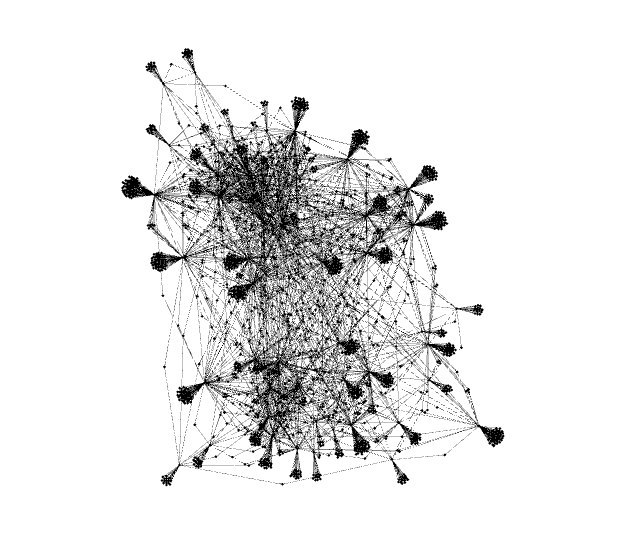
\includegraphics[width=0.8\textwidth]{jpg/swarm-topol.jpg}
      \caption*{Swarm network topology visualisation extracted by kabashira.}
      \label{fig:swarm-topol}
    \end{figure}
    
    The repo is \href{https://app.radicle.xyz/nodes/iris.radicle.xyz/rad%3Az41Aa98xcURaZQnV2Lrio1SoX3Tjd/tree/exotic-fleet-architectures.md}{hosted on Radicle}.
\end{enumerate}

\section*{Project management}

\subsection*{Completed Milestones}

\begin{itemize}
  \item Deliver recommendations to Swarm Foundation on protocol improvement process.
\end{itemize}

\subsection*{Next milestones}

\begin{itemize}
  \item Finalise SWIPs for stake withdrawals, stake record management, and adjacent changes.
  \item Revisiting storage pricing: performance analysis of price oracle and generation of alternative solutions.
  \item Seek community alignment on elements of economic and protocol roadmap.
\end{itemize}

\subsection*{Later milestones}
\begin{itemize}
  \item Migration-free stake registry: triage and concrete proposal.
  \item Negative incentives: explore and evaluate solutions.
  \item Empirical study of node strategies.
  \item Consensus attacks: analyse variants, evaluate threat level, list mitigations.
  \item Node dispersion: build mathematical model for address allocation schemes and node dispersion.
\end{itemize}


\subsection*{Roadmap highlights}

\paragraph{February}
%
Sync with Research team on BZZ value prop and tokenomics aspects of protocol roadmap.
%
Seek feedback on stake registry update queue semantics.
%
Scope out work to revisit storage price quoting mechanism.

\paragraph{March}
%
Subject to approval, begin work on price quoting mechanism.
%
Finalise alignment on protocol goals and priorities — both service reliability and value accrual.
%
Push for deployment of withdrawals changes during this month.

\subsection*{Roadmap changes}

Most of the research work of the Swarmonomics programme has been deprioritised in favour of more fundamental strategic and operational tasks: aiding the Swarm Foundation pin down protocol objectives and a process for reaching them.
%
This work is essential for operationalising our research work by putting needed protocol changes into production.

\section*{Current work}

Many of the current threads are yet to be published.
%
Here is a sneak preview:

\subsection*{Economic roadmap}

Our view is that Swarm's protocol roadmap needs to be driven by the following three principles:
%
\begin{enumerate}
  \item Stay true to the mission.
  \item Scale adoption.
  \item Scale investment.
\end{enumerate}
%
We aim to build community alignment on these principles and their consequences in the coming months (Q1 2026).

\paragraph{Scaling adoption} The part of scaling adoption that falls within the remit of economic analysis and protocol development is to \textbf{improve the service}.

Improving the service consists of chasing two objectives: \emph{improve reliability, reduce prices}.
%
These objectives naturally trade off against one another.
%
They should be prioritised as follows:
%
\begin{enumerate}
  \item \emph{improve reliability} to at least the level that meets the needs of target consumers;
  \item \emph{reduce prices}, given the reliability criteria, to a level that makes it competitive with its nearest alternatives.
\end{enumerate}

Reliability means a number of things:
%
\begin{itemize}
  \item 
    Availability: the service is available and able to deliver at threshold performance nearly all of the time.
    %
    Performance is part of availability — the service \emph{must} be fast enough to meet the target consumer's needs.
  \item 
    Durability: in the rare cases where the service does become unavailable, when it comes online again, all the data that is supposed to be available is still available.
  \item 
    Pricing: pricing is predictable enough that customers can reliably budget their use of the service.
\end{itemize}
%
These criteria are measurable: reliability and durability can be measured by consistent performance testing, and pricing predictability can be proxied by statistical measures like variance and IQR.

\paragraph{Reliability and incentives}
%
Swarm is Kademlia with financial incentives.
%
Financial incentives add significant complexity; to justify this, they \emph{must} fulfil their purpose of making Swarm reliable and scalable.
%
Swarm \emph{must} work even if no one operates nodes `altruistically'.

Key reliability properties:
\begin{enumerate}
  \item \emph{High quality service node population.} 
    Nodes should reliably store and serve data. 
    %
    Since we should not rely on altruistic nodes, we should measure this in terms of nodes that provide these services in exchange for payment.
    %
    Non-staking nodes operated by the Foundation and its partners must be explicitly excluded from this measure.
    
    An important proxy measure of storage service reliability is the \emph{participation rate}, that is, the number of successful storage proofs revealed each epoch. 
    %
    It is supposed to be 4 per round, or about 455 per day.
    %
    A drop in participation rate is an availability failure.

  \item 
    \emph{Provider failure tolerance.} Also known as censorship resistance.
    
    This is a question of \emph{Sybil resistance} and \emph{operator diversity}. 
    %
    If it's too cheap to force changes to the storage index, and hence alter the Swarm Network's commitments to store data, then Swarm is not censorship-resistant.
    %
    If all or nearly all nodes are operated by one entity, then no matter how many individual node identities there are, the service has a single point of failure.
    
  \item 
    \emph{Admin failure tolerance.} 
    %
    Alternatively, can the Foundation rug?
    
    The Swarm Network should continue to exist in the face of an absentee or even malicious Swarm Foundation.
    %
    Realistically, Swarm currently depends on the Foundation for continued maintenance and development, and likely will for some time.
    %
    Despite this, there are still ways that the Foundation can reduce its ability to exercise control over the protocol — most critically, it can be made impossible for the Foundation to steal or trap staker funds.

  \item 
    \emph{Capacity scaling.} That is, reliability in the face of scaling demand. 
    %
    Swarm should seek to vastly expand the raw capacity exposed by the network, ensuring a node population ready to handle a big demand spurt.
    %
    We should set an explicit capacity target, such as ``100TiB by H2 2026.''

\end{enumerate}

\paragraph{Scaling investment} is about communication, but it's also about improving token holder access to a slice of Swarm's success.
%
A BZZ investment should be \emph{aligned} with Swarm, in the sense that it pays off if and only if Swarm succeeds, by some defined measure of success.
%
In other words, a BZZ investment should win exactly when Swarm \emph{grows adoption given the constraints of its mission}.

The classical method to link an investment to the success of its object is to distribute profits to the investors.
%
The measure of success in this case is therefore \emph{profit}.

We will seek the Community's alignment on the following three assertions:
%
\begin{enumerate}
\item Cashflow is a firmer foundation for long-term value accrual than memetic consensus.
\item Staked BZZ has a cashflow: it is the capacity rental (stamp batch) reveneue.
\item It is not fundamental to the value proposition of BZZ that BZZ be used for payments.
\end{enumerate}
%
These principles inform the Shtuka Research position on BZZ value accrual, as communicated in previous reports: the golden path for delivering value to BZZ holders is to \emph{scale tokenholder access to storage revenue}.



\subsection*{Deciding on and communicating protocol changes}

The Swarm Protocol is the set of things a software system must do in order to participate in Swarm.
%
Unfortunately, it has historically been quite difficult for non-insiders to find out details about what the protocol actually is.
%
While the \href{https://papers.ethswarm.org/p/book-of-swarm/}{Book of Swarm} serves to define the scope of the protocol as a series of `layers' and introduce the ideas behind it, the book format is not suited to tracking a living protocol; indeed, many protocol changes have been made since the book was written.

We spent some time investigating how protocol decisions are made, how they are communicated, and explored avenues to improvement.

\paragraph{What parts make up the Swarm Protocol?}
Broadly speaking, each component of the Swarm Protocol falls into one of the following classes:
%
\begin{itemize}
  \item Peer-to-peer component — wire protocol.
  \item Peer-to-chain component — smart contracts and commitments, itself comprising:
  \begin{itemize}
    \item Node-facing component — stake registry and revenue redistribution.
    \item App-facing component — storage quota sales, tracking, and pricing.
  \end{itemize}
\end{itemize}
%
At Shtuka Research, we mainly work with the peer-to-chain protocol.

\paragraph{Who needs to know what the protocol is?} Protocol changes need to be flagged and communicated to a few groups of key stakeholders. 
%
In approximate order of priority:

\begin{itemize}
\item Foundation-internal (research and bee teams)
\item Builders (a.k.a. users)
\item Node operators, stakers
\item Alt client teams (e.g. browser client)
\item Protocol research partners (e.g. Shtuka)
\item Token holders  
\end{itemize}

Different parts of the protocol are relevant to different stakeholders:

\begin{itemize}
\item Postage or pricing changes $\rightarrow$ builders, node operators, client teams, protocol researchers.
\item Staking or redistribution changes $\rightarrow$ node operators, client teams, protocol researchers.
\item Wire protocol $\rightarrow$ client teams, protocol researchers, node operators (e.g. if new metric sharing is introduced), builders (e.g. if privacy properties are affected).
\end{itemize}

\paragraph{How are these changes being communicated now?} We did a search of multiple sources over the past year:

\begin{itemize}
\item Bee release notes
\item Bee PRs
\item SWIPs PRs
\item storage-incentives PRs
\item Foundation blog development update
\item Official documentation
\end{itemize}

We found that different types of protocol change are currently communicated in different places: 
%
\begin{itemize}
\item Bee PRs contain information about wire protocol changes, but these are buried among a much larger volume of bugfixes. Some wire protocol changes are marked \emph{Breaking} in bee release notes.
\item Storage-incentives PRs contain information about smart contract changes. The latter are in many cases accompanied by a SWIP.
\item The Foundation blog posts lack important details and the documentation, though constantly improving, is still often wrong.
\end{itemize}
%
Unsurprisingly, different sources end up disagreeing about protocol details, as illustrated by the following examples:

\begin{example*}[Reducing committed stake]

  The only onchain protocol change deployed last year was a fix to prevent \code{committedStake} from decreasing. 
  %
  It is recorded in an Issue and matching PR to the storage-incentives repo.

  Although the change affects the semantics of staking and the set of things node operators can do, it was not communicated in:
  %
  \begin{itemize}
  \item The SWIPs repo;
  \item The bee PR that implemented the new contract references;
  \item Bee release notes;
  \item The Foundation blog.
  \end{itemize}
  %
  The fact that \code{committedStake} cannot be decreased is not documented anywhere other than the merged PR on the storage-incentives repo.

\end{example*}

\begin{example*}[Overlay address derivation]

The derivation of overlay addresses was apparently changed between when Book of Swarm was published and the first mainnet deployment of the smart contracts.
%
Definitions diverge across different sources:

\begin{itemize}
\item The Book of Swarm defines it as a function of the pubkey associated to an Ethereum address and the Swarm network ID.
\item The \href{https://docs.ethswarm.org/docs/references/glossary/#overlay-address}{glossary} of the official documentation defines it in terms of the address itself and the network ID.
\item \href{https://docs.ethswarm.org/docs/bee/bee-faq/#can-i-use-one-ethereum-addresswallet-for-many-nodes}{Another section of the docs} mentions the nonce in a side remark.
\item The \href{https://papers.ethswarm.org/p/swarm-formal-spec/}{formal spec} give the full definition, including nonce and (little-endian) encoding of the network ID.
\item The AI helper on the official docs site says it doesn't know.
\end{itemize} 

As one would hope, the computation in the smart contracts matches the formal spec. 

This fundamental topic concerns essentially all participants in the Swarm ecosystem, yet it still seems to be hard to find out the current definition.

\end{example*}

\subsection*{Stake withdrawals and stake record update queue}

We've made substantial clarifications on our SWIPs 40 and 41, which now clearly specify changes to the interface and semantics of the Stake Registry to be implemented.
%
In our opinion, the architectural questions surrounding the new queue structure for tracking updates are now solved: the stake registry interface remains largely unchanged, but instead of reading directly from the stake table, getter functions apply pending updates in memory and return an up-to-date record.
%
The remaining point of contention is the queue semantics, which are largely an orthogonal question.

SWIP-41 calls for a per-owner FIFO queue in which each item is assigned a \emph{minimum delay}, according to a classification based on how substantial a commitment change it represents.
%
The delays serve dual purposes of \textbf{signalling} and \textbf{filtering} — it forces nodes that wish to change their commitments to signal the change in advance, giving the market time to react, and it filters out some churn based on short-term incentives like selling stake into a BZZ pump.

\paragraph{Ordering} The FIFO ordering rule is chosen for reasons of simplicity: it is the simplest type of queue to implement and it is easy to reason about.
%
Allowing out-of-order execution is not the default — we find that it should only be implemented if there is a compelling reason for it.

We do find a compelling reason to allow the updates associated to different owners to execute out of order — after all, why should one node's token deposit wait for another to exit an unrelated neighbourhood?

On the other hand, allowing out of order execution between updates to the same record is a recipe for contention.
%
For example, if a node operator enqueues a height decrease (exits a neighbourhood $\Rightarrow$ likely wants a longer delay) followed by a height increase (shorter delay), out of order execution could mean the first update overwrites the second — a race condition.
%
Similar scenarios arise for sequences of stake topups and drawdowns.

\paragraph{Throttling and complex queueing rules}
%
Discussions have also floated more complex queueing rules as possible improvements to the simple ``minimum delay'' principle underlying SWIP-41.
%
Many of these have complex state tracking requirements and a much larger design space, hence their omission from SWIP-41.
%
\begin{itemize}
  %
  \item 
    A global throttle on number of neighbourhood exits per round.
    %
    (A neighbourhood exit occurs when a node withdraws its commitment to host chunks in that address range.
    %
    Currently, nodes may exit a neighbourhood by reducing height or changing overlay; if SWIP-40 is implemented, they will also be able to withdraw a node completely.
    %
    An exception could be made for overlay changes, which do not reduce the overall storage commitment — they simply transfer it.)

  \item
    Fast lane for overlay changes that would move commitments from overserved into underserved address ranges.

\end{itemize}


\begin{figure}[h]
  \centering
  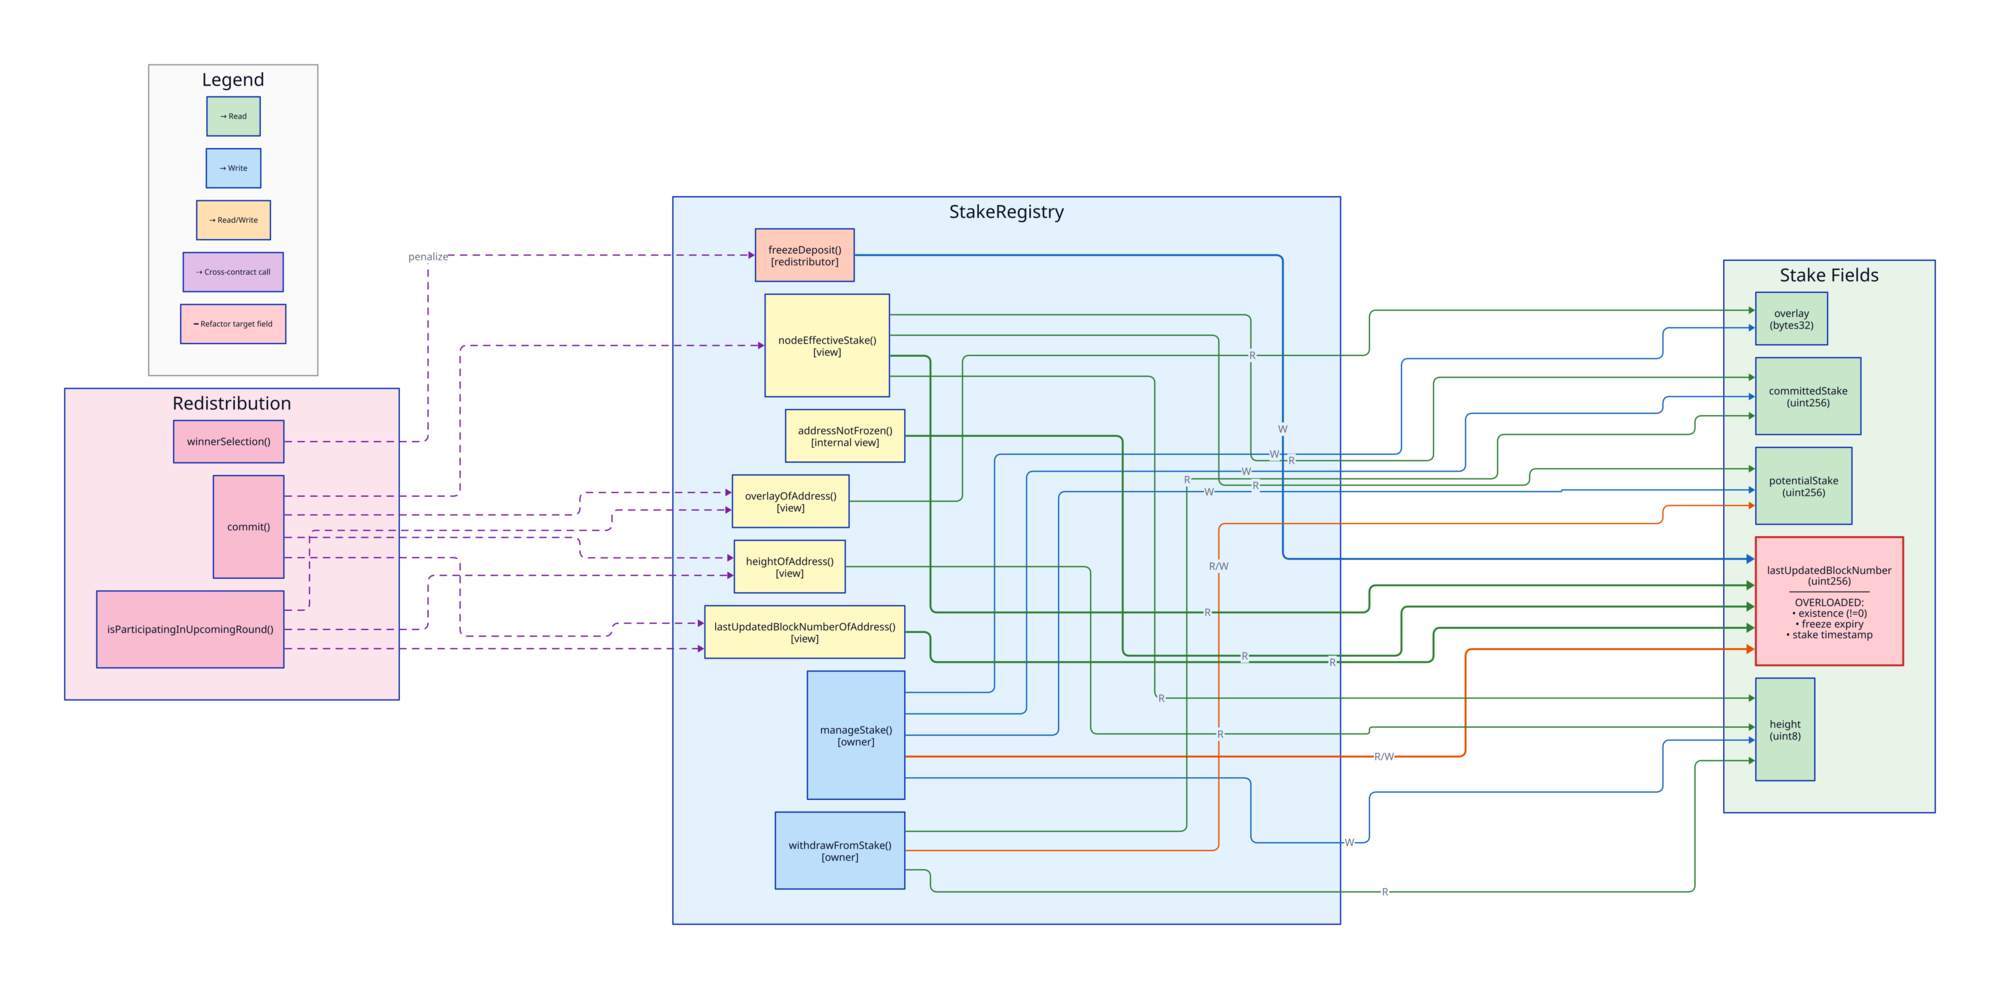
\includegraphics[width=0.95\textwidth]{png/stake-bipartite.png}
  \caption*{Simplified flow diagram of stake record management interfaces as they exist now}
\end{figure}